%!TEX root = doc.tex
\documentclass[twoside,10pt,parskip=half,ngerman]{scrreprt}

%***********************************************************************
% include some libs
%***********************************************************************
\usepackage[utf8]{inputenc}
\usepackage{listings}
\usepackage{xcolor}
\usepackage{color}
\usepackage{fancyhdr}
\usepackage{rotating}
\usepackage{titlesec}
\usepackage{mathptmx}
\usepackage{amssymb} % checkmark
% \usepackage{helvet}
\usepackage[scaled]{uarial}
\renewcommand*\familydefault{\sfdefault} %% Only if the base font of the document is to be sans serif
\usepackage[T1]{fontenc}
\usepackage[ngerman]{babel}
\usepackage[pdfauthor={Thomas Bandixen}, pdftitle={Bachelor-/Projektarbeit FS14 Studiengang Informatik - Projekttitel}, colorlinks=true,linkcolor=black,citecolor=black,plainpages=false]{hyperref}
\usepackage{textcomp}
\usepackage[squaren]{SIunits}
\usepackage{graphicx}
\usepackage{url}
\usepackage{geometry}
\usepackage[absolute]{textpos}
\usepackage{makeidx}
\usepackage{colortbl}
\usepackage{pdflscape}
\usepackage{pdfpages}
\usepackage{tabularx}
\usepackage{lmodern}
\usepackage{longtable}
\usepackage{array}
\usepackage{float}
\usepackage{scrhack}
\usepackage{wallpaper} %\ThisTileWallPaper{}
\usepackage[super,square]{natbib} %für BibTeX Literaturverzeichnis
\usepackage{packages/usecases}
% Glossar
\usepackage{footnote}
\makesavenoteenv{description}
\usepackage[acronym,section=section]{glossaries}
\renewcommand*{\glsentryfmt}{\ifglsused{\glslabel}{\glsentryname{\glslabel}}{\glsentrydesc{\glslabel}\space(\glsentryname{\glslabel})}}
\makeglossaries

%***********************************************************************
% various styles
%***********************************************************************

%create index
\makeindex

%define pagestyle
\pagestyle{fancy}

%use sans-serif font
%\renewcommand{\familydefault}{\sfdefault}

%define page margin
\geometry{a4paper, top=30mm, left=30mm, right=30mm, bottom=30mm,headsep=10mm,footskip=10mm}

%textpos parameter
\setlength{\TPHorizModule}{30mm}
\setlength{\TPVertModule}{\TPHorizModule}
\textblockorigin{10mm}{10mm} % start everything near the top-left corner
\setlength{\parindent}{0pt}

%horizontal lines for titlepage
\newcommand{\HRule}{\rule{\linewidth}{0.5mm}}

%reference to source items inlc source number
\newcommand{\srcref}[1]{\nameref{src:#1} \cite{#1}}

%header / footer
\renewcommand{\headrulewidth}{0.3pt}
\renewcommand{\footrulewidth}{0.3pt}

\fancyhead[LO,RE]{} %clear headings for contents
\fancyhead[RO,LE]{\nouppercase{\rightmark}} %right odd pages and left even pages
\fancyhead[LO,RE]{\MakeUppercase{\leftmark}} %left odd pages and right even pages
\fancyfoot[LE,RO]{\thepage} %page numbering
\fancyfoot[C]{} %clear centered page numbering

%define some colors
\definecolor{gray}{rgb}{0.95,0.95,0.95}
\definecolor{darkgray}{rgb}{0.4,0.4,0.4}
%listing colors
\definecolor{lgray}{RGB}{250,250,250}
\definecolor{lgreen}{RGB}{63,127,95}
\definecolor{lred}{RGB}{127,0,85}
\definecolor{lblue}{RGB}{42,0,255}

%***********************************************************************
% listing
%***********************************************************************

\lstset{
		basicstyle=\small\ttfamily,
		frame=single,
		numbers=left,
		numberstyle=\tiny,
		%firstnumber=auto,
		numberblanklines=true,
		captionpos=b,
		extendedchars=true,
		float=ht,
		showtabs=false,
		tabsize=2,
		showspaces=false,
		showstringspaces=false,
		breaklines=true,
		%prebreak=\Righttorque,
		backgroundcolor=\color{lgray},
		keywordstyle=\color{lred}\bfseries,
		commentstyle=\color{lgreen}\ttfamily,
%		morekeywords={printstr, printhexln},
		stringstyle=\color{lblue},
		xleftmargin=0.5cm,
		xrightmargin=0.5cm
}

\lstloadlanguages{[Sharp]C}
%\lstdefinestyle{sharpc}{language=[Sharp]C, frame=lr} %, rulecolor=\color{blue!80!black}

%\lstdefinelanguage{xc}{
%     keywords={printstr, printhexln, attributes, class, classend, do, empty, endif, endwhile, fail, function, functionend, if, implements, in, inherit, inout, not, of, operations, out, return, set, then, types, while, use},
%     keywordstyle=\color{lred}\bfseries,
%     ndkeywords={},
%     ndkeywordstyle=\color{yellow}\bfseries,
%     identifierstyle=\color{black},
%     sensitive=false,
%     comment=[l]{//},
%     commentstyle=\color{lgreen}\ttfamily,
%     string=[l]{"},
%     stringstyle=\color{lblue}\ttfamily
%  }


\begin{document}
%!TEX root = ../doc.tex
\newglossaryentry{zhaw}{name=ZHAW,description=Zürcher Hochschule für Angewandte Wissenschaften}

\bibliographystyle{plainnat}

\title{Verbesserung der Benutzer Erfahrung der Kundschaft eines internationalen Velokuriers} % In header.tex nachtragen
\author{Nicolas Roos}

%!TEX root = ../doc.tex
\begin{titlepage}

% Logo
\ThisTileWallPaper{\paperwidth}{\paperheight}{images/logos/SoE.pdf} % {images/logos/*.pdf}

\begin{minipage}[b]{0.117\textwidth}
\hskip 0.05cm
\end{minipage}
\begin{minipage}[b]{0.91\textwidth}
\begin{tiny}.\end{tiny}\vskip 2.8cm
	{\huge

	% Projekt Name (max. 2 Zeilen)
	\textbf{\underline{Bachelor-/Projektarbeit}}\\
	\textbf{\underline{FS14 Studiengang Informatik}}\\

	% Projekt Titel (max. 4 Zeilen)
	Titel der Arbeit
	\vskip 0.5cm}

	\begin{minipage}[b]{0.27\textwidth}
	\hrule\vskip 0.5cm
		\textbf{Autoren}\\
		\\
	\end{minipage}
	\begin{minipage}[b]{0.03\textwidth}
	\hskip 0.5cm
	\end{minipage}
	\begin{minipage}[b]{0.7\textwidth}
	\hrule\vskip 0.5cm
		Vorname Name\\
		Vorname Name\\
	\end{minipage}

	\begin{minipage}[b]{0.27\textwidth}
	\hrule\vskip 0.5cm
		\textbf{Hauptbetreuung}\\
		\\
	\end{minipage}
	\begin{minipage}[b]{0.03\textwidth}
	\hskip 0.5cm
	\end{minipage}
	\begin{minipage}[b]{0.7\textwidth}
	\hrule\vskip 0.5cm
		Vorname Name\\
		Vorname Name\\
	\end{minipage}

	\begin{minipage}[b]{0.27\textwidth}
	\hrule\vskip 0.5cm
		\textbf{Nebenbetreuung}\\
		\\
	\end{minipage}
	\begin{minipage}[b]{0.03\textwidth}
	\hskip 0.5cm
	\end{minipage}
	\begin{minipage}[b]{0.7\textwidth}
	\hrule\vskip 0.5cm
		Vorname Name\\
		Vorname Name\\
	\end{minipage}

	\begin{minipage}[b]{0.27\textwidth}
	\hrule\vskip 0.5cm
		\textbf{Industriepartner}\\
		\\
	\end{minipage}
	\begin{minipage}[b]{0.03\textwidth}
	\hskip 0.5cm
	\end{minipage}
	\begin{minipage}[b]{0.7\textwidth}
	\hrule\vskip 0.5cm
		Firmenname\\
		\\
	\end{minipage}

	\begin{minipage}[b]{0.27\textwidth}
	\hrule\vskip 0.5cm
		\textbf{Externe Betreuung}\\
		\\
	\end{minipage}
	\begin{minipage}[b]{0.03\textwidth}
	\hskip 0.5cm
	\end{minipage}
	\begin{minipage}[b]{0.7\textwidth}
	\hrule\vskip 0.5cm
		Vorname Name\\
		Vorname Name\\
	\end{minipage}

	\begin{minipage}[b]{0.27\textwidth}
	\hrule\vskip 0.5cm
		\textbf{Datum}
	\end{minipage}
	\begin{minipage}[b]{0.03\textwidth}
	\hskip 0.5cm
	\end{minipage}
	\begin{minipage}[b]{0.7\textwidth}
	\hrule\vskip 0.5cm
		\today
	\end{minipage}
\end{minipage}
\vskip 0.5cm


\textcolor{darkgray}{
Bitte füllen Sie das Titelblatt aus und berücksichtigen Sie Folgendes:\\
 -> Bitte auf keinen Fall Schriftart und Schriftgrösse ändern. Text soll lediglich überschrieben werden!\\
 -> Bitte pro Tabellenzeile max. 4 Textzeilen!\\
\\
•	Titel: Fügen Sie Ihren Studiengang direkt nach dem Wort „Bachelorarbeit“ ein (max. 2 Zeilen).\\
•	Titel der Arbeit: Überschreiben Sie den Lauftext mit dem Titel Ihrer Arbeit (max. 4 Zeilen).\\
•	Autoren: Tragen Sie Ihre Vor- und Nachnamen ein (alphabetisch nach Name).\\
•	Betreuer: Tragen Sie Ihren Betreuer / Ihre Betreuer ein (alphabetisch nach Name).\\
•	Ohne Nebenbetreuung, Industriepartner oder externe Betreuung, ganze Tabellenzeile löschen.\\
•	Am Schluss löschen Sie den ganzen Beschrieb (grau) und speichern das Dokument als pdf. ab.
}

\end{titlepage}

\setcounter{page}{1}
%!TEX root = ../doc.tex
\thispagestyle{empty}
\chapter*{Zusammenfassung}
\label{sec:Zusammenfassung}
\textcolor{darkgray}{
  Zusammenfassung
}

\chapter*{Vorwort}
\label{sec:Vorwort}

\textcolor{darkgray}{
  Stellt den persönlichen Bezug zur Arbeit dar und spricht Dank aus.
}


% 
\includepdf{images/Erklaerung_PA.pdf} % Entsprechendes auskommentieren

\includepdf{images/Erklaerung_BA.pdf}
% \newpage

%Inhaltsverzeichnis
\tableofcontents
\newpage

%\textbf{}
%\setcounter{page}{1}
%\pagenumbering{arabic}

%!TEX root = ../doc.tex
\chapter{Einleitung}
\label{sec:Einleitung}

\section{Ausgangslage}
\label{sec:Ausgangslage}

\textcolor{darkgray}{
  \begin{itemize}
  \item Nennt bestehende Arbeiten/Literatur zum Thema -> Literaturrecherche
  \item Stand der Technik: Bisherige Lösungen des Problems und deren Grenzen
  \item (Nennt kurz den Industriepartner und/oder weitere Kooperationspartner und dessen/deren Interesse am Thema Fragestellung)
  \end{itemize}
}

\section{Zielsetzung / Aufgabenstellung / Anforderungen}
\label{sec:ZielsetzungAufgabenstellungAnforderungen}

\textcolor{darkgray}{
  \begin{itemize}
  \item Formuliert das Ziel der Arbeit
  \item Verweist auf die offizielle Aufgabenstellung des/der Dozierenden im Anhang
  \item (Pflichtenheft, Spezifikation)
  \item (Spezifiziert die Anforderungen an das Resultat der Arbeit)
  \item (Übersicht über die Arbeit: stellt die folgenden Teile der Arbeit kurz vor)
  \item (Angaben zum Zielpublikum: nennt das für die Arbeit vorausgesetzte Wissen)
  \item (Terminologie: Definiert die in der Arbeit verwendeten Begriffe)
  \end{itemize}
}
%!TEX root = ../doc.tex
\chapter{Recherche}
\label{sec:recherche}

\section{Kurier Business}
\section{Kurier und Logistik Software} % (2. Theoretische Grundlagen)
%!TEX root = ../doc.tex
\chapter{Ist Analyse}
\label{sec:istanalyse}

\section{Aktuelle Prozesse}
\section{Eingesetze Software bei ImagineCargo} % Vorgehen / Methoden
%!TEX root = ../doc.tex
\chapter{User Centered Design}
\label{sec:usercentric}
Als \textit{User Centered Design} werden Prinzipien und Werkzeuge verstanden, welche den Designern, Entwicklern und allen anderen die an der Entstehung eines Produktes, Services oder Prozesses beteiligt sind, helfen die Bedürfnisse und Wünsche des Endbenutzer während der gesamten Entwicklungsphase mit hoher Priorität in den Vordergrund zu stellen. Dieses Framework steht in starkem Kontrast zu herkömmlichen Entwicklungsmethoden bei welchen die Stakeholders zu einem grossen Teil die Ausrichtung, das Aussehen und Verhalten einer neuen Erschaffung bestimmen. Bei diesen älteren Entwicklungsmethoden kam es vermehrt dazu, dass ein Produkt erst bei der Veröffentlichung zum ersten mal die Hände eines Endbenutzer berührte und sich dann als komplett unnütz herausstellte. Der \textit{User Centered Design} Ansatz involviert mögliche Endbenutzer bereits ab den ersten Entwicklungsphasen und fordert dadurch das Zielpublikum zur Mitgestaltung auf. Dadurch werden viele Probleme die bei einer Markteinführung auftreten können, bereits früh entdeckt und behoben. Die Anwendung dieses Frameworks kostet im Gegensatz zu anderen Methoden mehr Zeit und dadurch auch mehr Geld. \textit{User Centered Design} ist eine iterative Methode, welche nach der Durchführung ihrer Teilschritte wieder von vorne beginnt. In Abbildung \ref{fig:usercentereddesign} ist eine mögliche schematische Darstellung des Ablaufs von \textit{User Centered Design}.

\begin{figure}[ht]
	\centering
  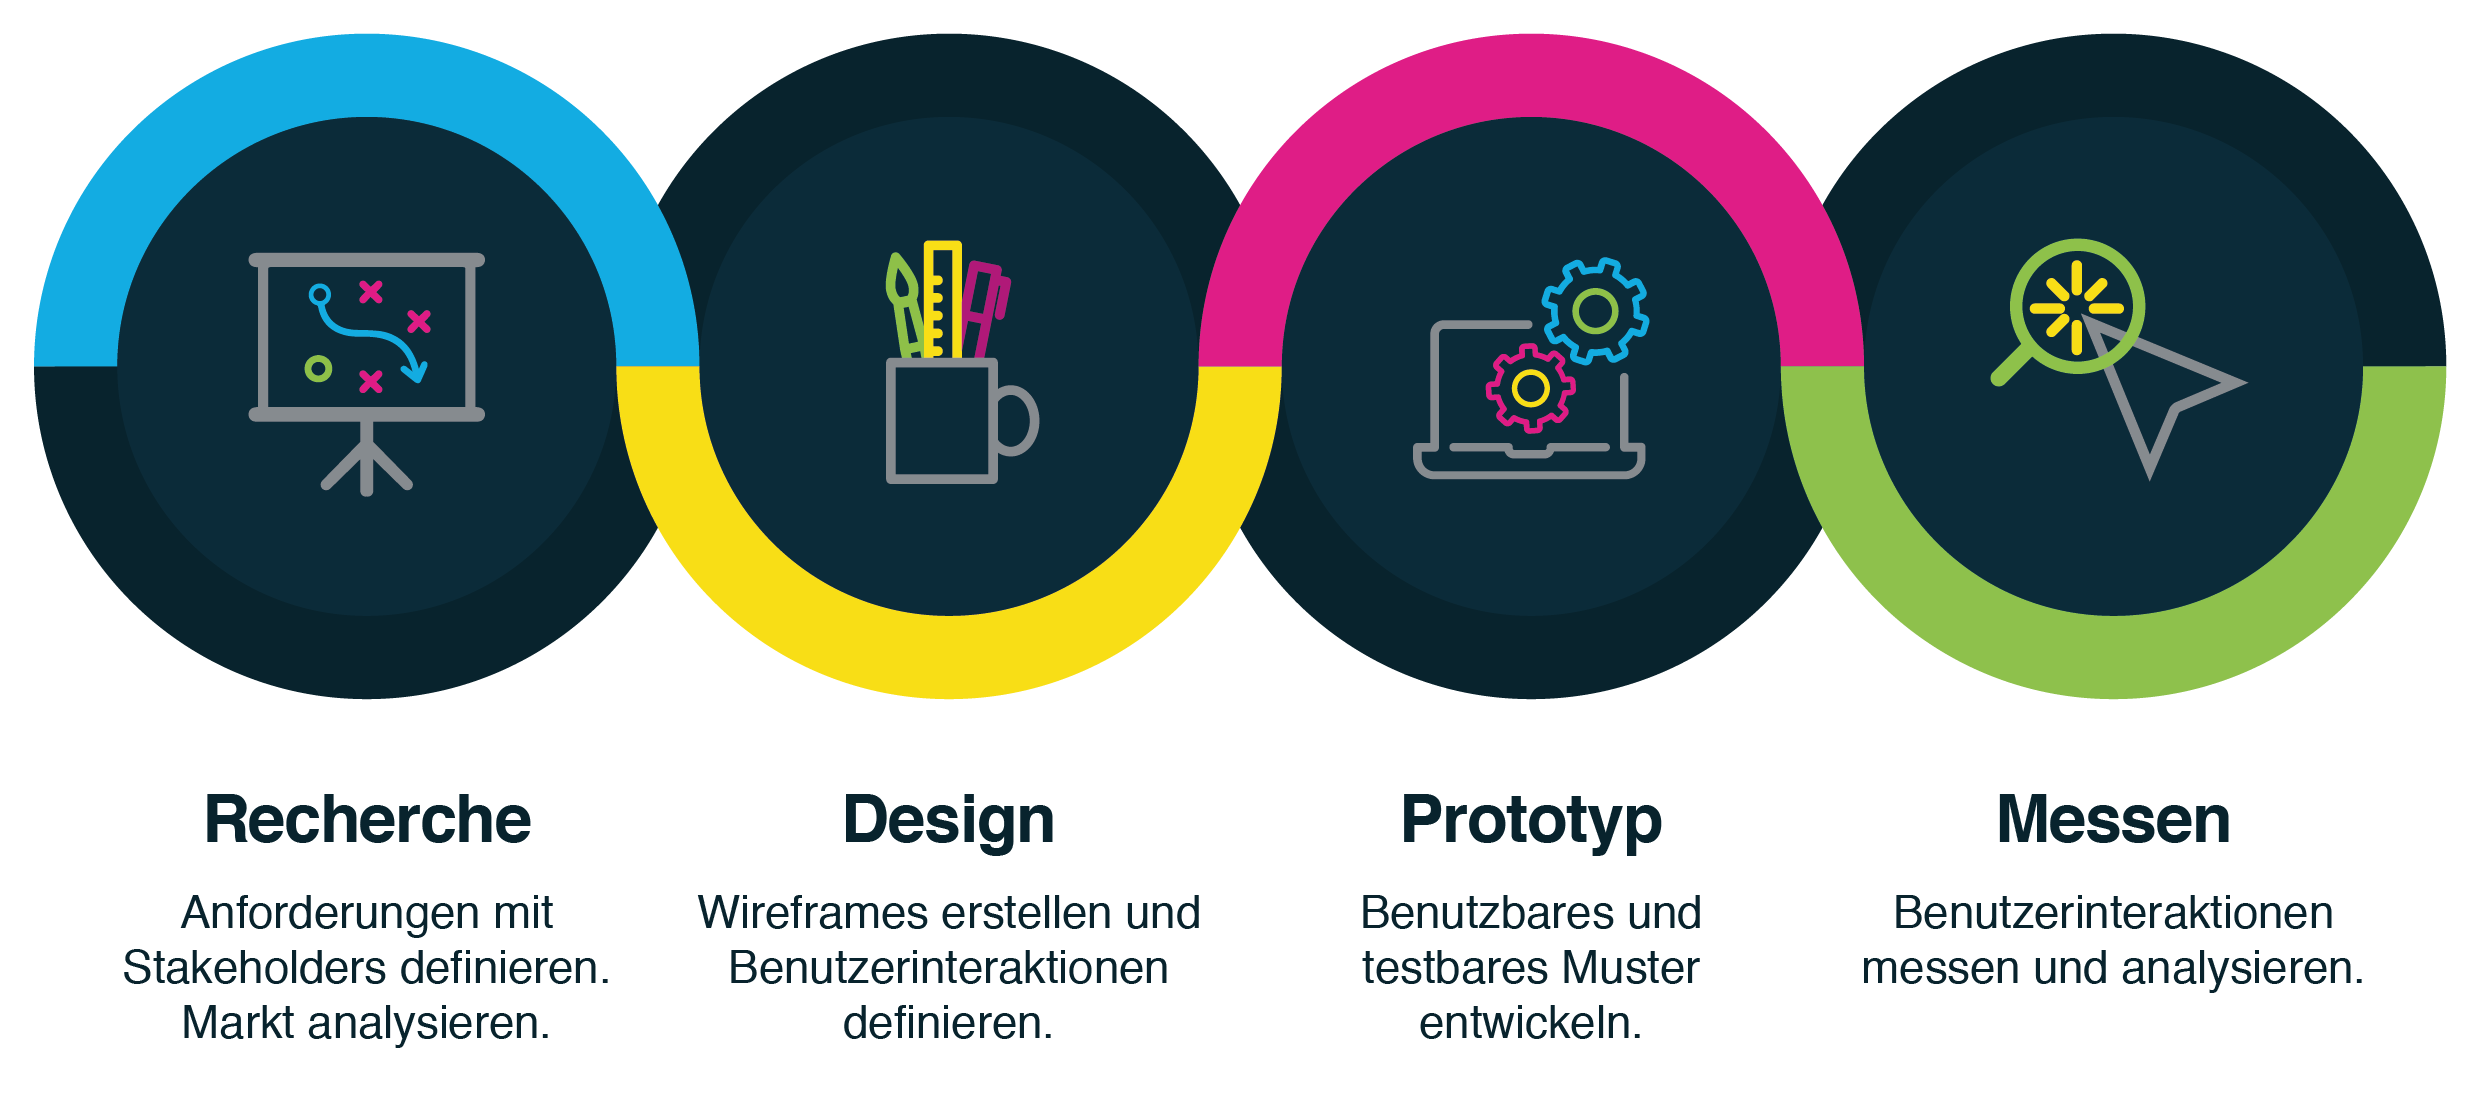
\includegraphics[width=0.88\textwidth]{images/userCenteredDesign.png}
	\caption{Prozessablauf von User Centered Design}
	\label{fig:usercentereddesign}
\end{figure}

Während all diesen Teilschritten werden die Ergebnisse und Erkenntnisse den möglichen Endbenutzern vorgestellt. Dabei wird überprüft ob z.B. der Interaktionsfluss oder die Benutzeroberflächen einer Applikation verständlich ist oder alle relevanten Spezialfälle abdeckt. \textit{User Centered Design} kann auf viele verschiedene Arte angewendet werden und zu den gewünschten Resultaten führen. Diese Bachelorthesis orientiert sich am User Centered Design Ablauf welcher im Buch von Kim Goodwin mit dem Namen \textit{Designing for the Digital Age}\citep{goodwin2011designing} beschrieben wird.


\section{Anwendung}
In den ersten Gesprächen mit den Stakeholdern wurde schnell klar, dass das Ziel des Produktes eine Webapplikation sein soll, welche von Benutzer jeglicher Generation und Demographie benutzt werden kann. Die Entscheidung für eine Entwicklung unter \textit{User Centered Design} war naheliegend. Im folgenden ist der geplante Ablauf mit dem Fokus auf den Endbenutzer beschrieben.

\subsection{Team}
Bei der Zusammenstellung des Design Teams ist es wichtig die verschiedenen benötigten Fähigkeiten in einer kleinen Gruppe zusammen zu fassen. Ein Interaktions Designer hat einen ganz anderen Fokus als der Grafische Designer. Im Rahmen dieser Bachelorthesis fielen alle Rollen des Designs auf eine Person. Diese Konstellation ist nicht per se benachteiligt. Diese einzelne Person muss aber in der Lage sein während den verschiedenen Phasen die Probleme, Ideen, Vorschläge, Lösungen und vieles andere aus den jeweiligen Perspektiven zu betrachten und beurteilen. In der idealen Zusammensetzung nach Goodwin sind folgende Rollen zu besetzen\citep[Kapitel 2]{goodwin2011designing}.
\begin{description}
	\item [Teamleiter\_in] Verantwortlich für das Team und die Koordination mit allen anderen involvierten.
	\item [Interaction Designer\_in (Generator)] Verantwortlich für die Visualisierung des Systemverhalten
	\item [Interaction Designer\_in (Synthesizer)] Verantwortlich für die Analyse und Kommunikation des Designs.
	\item [Grafischer Designer\_in] Verantwortlich für die Visuelle Umsetzung des Designs.
	\item [Industrie Designer\_in] Verantwortlich für das Design der Hardware.
\end{description}

\subsection{Grundlegende Recherche der Domäne}
Während der Recherche wird die Domäne in welcher sich das zu erschaffende Produkt befindet analysiert. Dabei werden Marktanalysen getätigt sowie falls vorhanden die Produkte der Konkurrenz untersucht. Zusätzlich werden Experten und Menschen welche bereits lange in dem Bereich tätig sind befragt. Diese Arbeit wird vom gesamten Design Team bewältigt da bereits in dieser Phase die verschiedene Perspektiven wichtig sind. Mit Nick Blake als Gründer von Imagine Cargo und Experte der Kurier-, Express- und Paketdienst Industrie hat diese Bachelorthesis auf sehr viel Erfahrung und Insiderwissen zurückgreifen können.

\subsection{Interviews mit Stakeholders}
Bevor Interviews beginnen können müssen die Stakeholders zuerst definiert werden. Zu den Stakeholders gehören grundsätzlich alle Menschen die ein Produkt mit bestimmen können. Jedoch zählt nicht jede Meinung gleich viel. Bei der Analyse ist es wichtig mit allen involvierten Menschen zu reden und auch die Personen ausfindig machen, welche sich aus dem ganzen Design Prozess raus halten aber die Macht haben das ganze Projekt zu beerdigen. Üblicherweise finden sich solche Stakeholders im Management die das Gefühl haben ihre Meinung sei noch nicht notwendig bzw. er/sie werde erst aktiv wenn das Projekt ein Fundament hat. Meist ist es dann aber zu spät für Grundlegende Designänderungen. Für die Bachelorthesis wurden David Emmerth und Nick Blake von Imagine Cargo interviewt. Die Fragen für die Interviews sind vom Buch von Kim Goodwin inspiriert worden\citep[Kapitel 5]{goodwin2011designing} und sind im Anhang \ref{subsec:stakeholderfragen} zu finden. Die Zusammenfassungen der Interviews sind in Kapitel \ref{sec:interviews} nach zu lesen.

\subsection{Interviews mit Endbenutzer}
In den Interviews mit den Stakeholdern sollte sich eine grobe Definition des zu erstellenden Produktes heraus kristallisieren. Mit dieser gewonnen Definition werden mit möglichen Endbenutzern Interviews geführt, welche weitere Einblicke in die Anforderungen und Unzufriedenheiten mit bestehenden Produkten zu Tage bringt. Aufgrund der beschränkten Ressourcen die dieser Bachelorthesis zur verfügung stehen, wurde auf diesen Schritt verzichtet. In der Visualisierungs Phase sollen die erstellten Wireframes und den Interaktionsablauf mit möglichen Endbenutzern überprüft werden.

\subsection{Personas}

%Personas erstellen \\
%Persona Stories erstellen & Anforderungen definieren \\





\section{Interviews}
\label{sec:interviews}
\textcolor{darkgray}{
	Beschreibung der geführten Interviews und den Gesprächspartnern
} % Vorgehen / Methoden
%!TEX root = ../doc.tex
\chapter{Anforerdungsanalyse}
\label{sec:anforderungsanalyse}

\section{Interview}
\section{User Centric? Usecases}
\section{freq}
\section{nfreq}
\section{akzeptanztests}




\begin{usecase}

\addtitle{Use Case 1}{Template test}

%Scope: the system under design
\addfield{Scope:}{System-wide}

%Level: "user-goal" or "subfunction"
\addfield{Level:}{User-goal}

%Primary Actor: Calls on the system to deliver its services.
\addfield{Primary Actor:}{End-User}

%Stakeholders and Interests: Who cares about this use case and what do they want?
\additemizedfield{Stakeholders and Interests:}{
	\item Stakeholder 1 name: his interests
	\item Stakeholder 2 name: his interests
}

%Preconditions: What must be true on start and worth telling the reader?
\addfield{Preconditions:}{}
%when multiple
%\additemizedfield{Preconditions:}{}

%Postconditions: What must be true on successful completion and worth telling the reader
\addfield{Postconditions:}{}
%when multiple
%\additemizedfield{Preconditions:}{}

%Main Success Scenario: A typical, unconditional happy path scenario of success.
\addscenario{Main Success Scenario:}{
	\item The first action
	\item The second action
}

%Extensions: Alternate scenarios of success or failure.
\addscenario{Extensions:}{
	\item[2.a] Invalid login data:
		\begin{enumerate}
		\item[1.] System shows failure message
		\item[2.] User returns to step 1
		\end{enumerate}
	\item[5.a] Invalid subsriber data:
		\begin{enumerate}
		\item[1.] System shows failure message
		\item[2.] User returns to step 2 and corrects the errors
		\end{enumerate}
}

%Special Requirements: Related non-functional requirements.
\additemizedfield{Special Requirements:}{
	\item first applicable non-functional requirement
	\item second applicable non-functional requirement
}

%Technology and Data Variations List: Varying I/O methods and data formats.
\addscenario{Technology and Data Variations List:}{
	\item[1a.] Alternative first action with other technology
}

%Frequency of Occurrence: Influences investigation, testing and timing of implementation.
\addfield{Frequency of Occurrence:}{}

%Miscellaneous: Such as open issues/questions
%\addfield{Open Issues:}{}

\end{usecase}
%!TEX root = ../doc.tex
\chapter{Konzept}
\label{sec:konzept}

\section{Planung}
\section{Schnittstellen}
\section{Technologie}
\section{Architektur}
\section{Go for Prototyp / no go for prototyp }
%!TEX root = ../doc.tex
\chapter{Prototyp}
\label{sec:prototyp}

\section{Entwicklungsprozess} % Diskussion und Ausblick
%!TEX root = ../doc.tex
\chapter{Test}
\label{sec:test}

\section{akzeptanztests}
\section{unittests}

%!TEX root = ../doc.tex
\chapter{Fazit}
\label{sec:fazit}

\section{???}

\chapter{Verzeichnisse}
\label{sec:Verzeichnisse}
\addcontentsline{toc}{section}{Literaturverzeichnis}
\bibliography{BibTeX/literatur}
\listoffigures
\addcontentsline{toc}{section}{Abbildungsverzeichnis}
\listoftables
\addcontentsline{toc}{section}{Tabellenverzeichnis}
%!TEX root = ../doc.tex
\chapter*{Glossar}
\label{sec:Glossar}
\addcontentsline{toc}{section}{Abkürzungsverzeichnis}\label{cha:abkürzungsverzeichnis}

In diesem Abschnitt werden Abkürzungen und Begriffe kurz erklärt.
\setglossarystyle{altlistgroup}
\printglossary[title=]


\lstlistoflistings
\addcontentsline{toc}{section}{Listingverzeichnis}

%!TEX root = ../doc.tex
\pagenumbering{Roman}

\appendix
\chapter{Anhang}
\label{sec:Anhang}

\section{Projektmanagement}\label{projektmanagement}

\textcolor{darkgray}{
  \begin{itemize}
  \item Offizielle Aufgabenstellung, Projektauftrag
  \item (Zeitplan)
  \item (Besprechungsprotokolle oder Journals)
  \end{itemize}
}

\section{Weiteres}
\label{sec:Weiteres}

\textcolor{darkgray}{
  \begin{itemize}
  \item CD mit dem vollständigen Bericht als pdf-File inklusive Film- und Fotomaterial
  \item (Schaltpläne und Ablaufschemata)
  \item (Spezifikationen u. Datenblätter der verwendeten Messgeräte und/oder Komponenten)
  \item (Berechnungen, Messwerte, Simulationsresultate)
  \item (Stoffdaten)
  \item (Fehlerrechnungen mit Messunsicherheiten)
  \item (Grafische Darstellungen, Fotos)
  \item (Datenträger mit weiteren Daten (z.B. Software-Komponenten) inkl. Verzeichnis der auf diesem Datenträger abgelegten Dateien)
  \item (Softwarecode)
  \end{itemize}
}


\end{document}
